\begin{frame}

\frametitle{Git: Workflow}

\begin{multicols}{2}
Git has three main states that your files can reside in:

\begin{itemize}[<+(1)->]
\item \textbf{Modified}
\item \textbf{Staged}
\item \textbf{Committed}
\end{itemize}

\columnbreak

git add file1 file2 dir1 dir2

git commit -m "Fancy feature done."


\end{multicols}

\begin{figure}
\centering
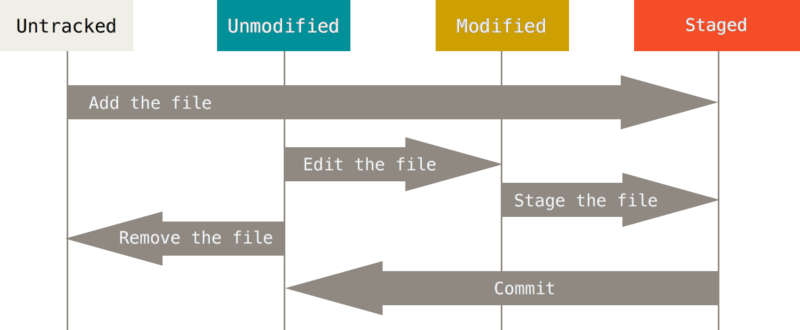
\includegraphics[scale=0.25]{git-lifecycle-file.png}
\caption{File lifecycle. From \href{https://git-scm.com/book/en/v2/Git-Basics-Recording-Changes-to-the-Repository}{Git SCM}}
\end{figure}

\end{frame}